\section{Points}
\subsection{Comparing floating point values}
Returns true if double values a and b are equal
\cppscript{geometry/src/equals}{equals}


\section{Lines}
\subsection{General equation of a line}
Non-normalized form: ax + by + c = 0
\cppscript{geometry/src/line_general}{General equation of a line}

\subsection{General equation of a line normalized}
\cppscript{geometry/src/line_general_normalized}{General equation of a line}

\subsection{Point on a line}
Is the given point located on the given Line?
\cppscript{geometry/src/line_contains}{Point on line}

\section{Vectors}

\subsection{Angle between vector and X-axis}
Returns an angle in radians in the interval $\interval{-\pi}{+\pi}$. A positive angle means in the COUNTER-clockwise direction. A negative angle is measured in the clockwise direction. Note that the atan2 swaped the parameters.
\cppscript{geometry/src/angle}{angle between X-axis and vector{x, y}}

\subsection{Translation}
\cppscript{geometry/src/translation}{Translate point}

\subsection{Rotation around origin}
\cppscript{geometry/src/rotation}{}

\subsection{Rotation around another point}
\cppscript{geometry/src/rotation_point}{}

\subsection{Rotation around origin 3D}

\begin{center}
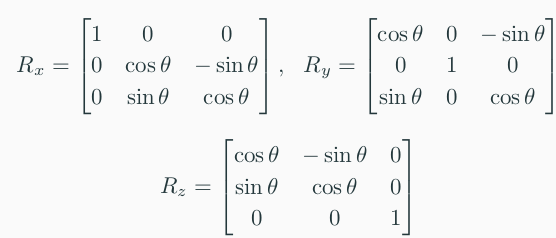
\includegraphics[width = 7in, height = 3.5in]{geometry/images/rotation3d.png}
\end{center}

\clearpage
